%---------------------------------------------------------------------------%
%-                                                                         -%
%-                           LaTeX Template                                -%
%-                                                                         -%
%---------------------------------------------------------------------------%
%- Copyright (C) Huangrui Mo <huangrui.mo@gmail.com> 
%- This is free software: you can redistribute it and/or modify it
%- under the terms of the GNU General Public License as published by
%- the Free Software Foundation, either version 3 of the License, or
%- (at your option) any later version.
%---------------------------------------------------------------------------%
%->> Document class declaration
%---------------------------------------------------------------------------%
\documentclass[oneside]{Style/ucasthesis}% [oneside, twoside]
%- Multiple optional arguments:
%- [<oneside|twoside|print>]% oneside eprint, twoside eprint, or paper print
%- twoside chapter start from odd page, but onesize does not.
%- [fontset=<adobe|none|...>]% specify font set instead of automatic detection
%- [scheme=plain]% thesis writing of international students
%- [draftversion]% show draft version information
%- [standard options for ctex book class: draft|paper size|font size|...]%
%---------------------------------------------------------------------------%
%->> Document settings
%---------------------------------------------------------------------------%
\usepackage[numbers,list]{Style/artratex}% document settings, authoryear
%- usage: \usepackage[option1,option2,...,optionN]{artratex}
%- Multiple optional arguments:
%- [bibtex|biber]% set bibliography processor and package
%- [<numbers|super|authoryear|alpha>]% set citation and reference style
%- <numbers>: textual: Jones [1]; parenthetical: [1]
%- <super>: textual: Jones superscript [1]; parenthetical: superscript [1]
%- <authoryear>: textual: Jones (1995); parenthetical: (Jones, 1995)
%- <alpha>: textual: not available; parenthetical: [Jon95]
%- [geometry]% reconfigure page layout via geometry package
%- [lscape]% provide landscape layout environment
%- [xhf]% disable header and footer via fancyhdr package
%- [color]% provide color support via xcolor package
%- [background]% enable page background
%- [tikz]% provide complex diagrams via tikz package
%- [table]% provide complex tables via ctable package
%- [list]% provide enhanced list environments for algorithm and coding
%- [math]% enable some extra math packages
%- [xlink]% disable link colors
%---------------------------------------------------------------------------%
%->> New command
%---------------------------------------------------------------------------%
\newcommand\norm[1]{\left\lVert#1\right\rVert}
\DeclareMathOperator{\dis}{d}
\usepackage{tabu}
\usepackage{multirow}
\usepackage{balance}

\usepackage{Style/artracom}% user defined commands
%---------------------------------------------------------------------------%
%->> Document inclusion
%---------------------------------------------------------------------------%
%\includeonly{Tex/Chap_1,...,Tex/Chap_N}% selected files compilation
%---------------------------------------------------------------------------%
%->> Document content
%---------------------------------------------------------------------------%
%-
%-> Titlepage information
%-
%---------------------------------------------------------------------------%
%->> Titlepage information
%---------------------------------------------------------------------------%
%-
%-> 中文封面信息
%-
\usepackage{amssymb}

\confidential{}% 密级:只有涉密论文才填写
%\schoollogo[scale=0.095]{ucas_logo}% 校徽
\title{学位论文中期考核报告}% 页眉题目
\casia{中国科学院自动化研究所}% 论文中文题目

\papertitle{笑傲江湖}


%\advisor{指导教师一\\指导教师二\\指导教师三}% 多行指导教师示例
\degree{博士}% 学位:学士、硕士、博士
\degreetype{理学}% 学位类别:理学、工学、工程、医学等

\major{模式识别与智能系统}% 二级学科专业名称
\submajor{计算机视觉}% 专业
\author{令狐冲}% 论文作者
\studentnumber{201818014628079}% 论文作者
\casiadegreetype{
	\makebox[0pt][l]{$\framebox(9,9){}$}\raisebox{.15ex}{\hspace{0.1em}$\checkmark$}博士\quad $\framebox(9,9){}$硕士
}% 论文作者

\studenttype{
	\makebox[0pt][l]{$\framebox(9,9){}$}\raisebox{.15ex}{\hspace{0.1em}$\checkmark$}硕博连读\quad
	$\framebox(9,9){}$直接攻博 \quad 
	$\framebox(9,9){}$普通招考
}% 论文作者

\advisor{风清扬}% 指导
\lab{智能系统与工程}% 指导
\currentdate{2020~年~12~月~11~日}% 指导

\institute{xxx}% 研究方向
%\institute{中国科学院力学研究所\\流固耦合实验室}% 多行院系名称示例
\date{2020~年~6~月}% 毕业日期:夏季为6月、冬季为12月
%-
%-> 英文封面信息
%-
\TITLE{\LaTeX{} Thesis Template\\ of \\ The University of Chinese Academy of Sciences {$~^{\pi}\pi^{\pi}$}}% 论文英文题目
\AUTHOR{Mo Huangrui}% 论文作者
\ADVISOR{Supervisor: Professor Liu Qingquan}% 指导教师
\DEGREE{Bachelor}% 学位:Bachelor, Master, Doctor, Postdoctor。封面据英文学位名称自动切换,需确保拼写准确
\DEGREETYPE{Natural Science}% 学位类别:Philosophy, Natural Science, Engineering, Economics, Agriculture 等
\MAJOR{Fluid Mechanics}% 二级学科专业名称
\INSTITUTE{Institute of Mechanics, Chinese Academy of Sciences}% 院系名称
\DATE{June, 2014}% 毕业日期:夏季为June、冬季为December
%---------------------------------------------------------------------------%
%

\begin{document}
%-
%-> Frontmatter: title page, abstract, content list, symbol list, preface
%-
\frontmatter% initialize the environment
%---------------------------------------------------------------------------%
%->> Frontmatter
%---------------------------------------------------------------------------%
%-
%-> 生成封面
%-
\maketitle% 生成中文封面
%\MAKETITLE% 生成英文封面
%-
%-> 作者声明
%-
%\makedeclaration% 生成声明页
%-
%-> 中文摘要
%-
%\intobmk\chapter*{摘\quad 要}% 显示在书签但不显示在目录
%\setcounter{page}{1}% 开始页码
%\pagenumbering{Roman}% 页码符号

%本文是中国科学院大学学位论文模板ucasthesis的使用说明文档。主要内容为介绍\LaTeX{}文档类ucasthesis的用法,以及如何使用\LaTeX{}快速高效地撰写学位论文。
%
%\keywords{中国科学院大学,学位论文,\LaTeX{}模板}% 中文关键词
%-
%-> 英文摘要
%-
%\intobmk\chapter*{Abstract}% 显示在书签但不显示在目录

%This paper is a help documentation for the \LaTeX{} class ucasthesis, which is  a thesis template for the University of Chinese Academy of Sciences. The main content is about how to use the ucasthesis, as well as how to write thesis efficiently by using \LaTeX{}.
%
%\KEYWORDS{University of Chinese Academy of Sciences (UCAS), Thesis, \LaTeX{} Template}% 英文关键词
%---------------------------------------------------------------------------%
% title page, abstract
{% content list region
\linespread{1.2}% local line space
\intobmk*{\cleardoublepage}{\contentsname}% add link to bookmark
\tableofcontents% content catalog
%\intobmk*{\cleardoublepage}{\listfigurename}% add link to bookmark
%\listoffigures% figure catalog
%\intobmk*{\cleardoublepage}{\listtablename}% add link to bookmark
%\listoftables% table catalog
}

%\intobmk\chapter*{符号列表}% 显示在书签但不显示在目录

\section*{字符}
\nomenclatureitem[\textbf{Unit}]{\textbf{Symbol}}{\textbf{Description}}
\nomenclatureitem[$\Unit{m^{2} \cdot s^{-2} \cdot K^{-1}}$]{$R$}{the gas constant}
\nomenclatureitem[$\Unit{m^{2} \cdot s^{-2} \cdot K^{-1}}$]{$C_v$}{specific heat capacity at constant volume}
\nomenclatureitem[$\Unit{m^{2} \cdot s^{-2} \cdot K^{-1}}$]{$C_p$}{specific heat capacity at constant pressure}
\nomenclatureitem[$\Unit{m^{2} \cdot s^{-2}}$]{$E$}{specific total energy}
\nomenclatureitem[$\Unit{m^{2} \cdot s^{-2}}$]{$e$}{specific internal energy}
\nomenclatureitem[$\Unit{m^{2} \cdot s^{-2}}$]{$h_T$}{specific total enthalpy}
\nomenclatureitem[$\Unit{m^{2} \cdot s^{-2}}$]{$h$}{specific enthalpy}
\nomenclatureitem[$\Unit{kg \cdot m \cdot s^{-3} \cdot K^{-1}}$]{$k$}{thermal conductivity}
\nomenclatureitem[$\Unit{kg \cdot m^{-1} \cdot s^{-2}}$]{$S_{ij}$}{deviatoric stress tensor}
\nomenclatureitem[$\Unit{kg \cdot m^{-1} \cdot s^{-2}}$]{$\tau_{ij}$}{viscous stress tensor}
\nomenclatureitem[$\Unit{1}$]{$\delta_{ij}$}{Kronecker tensor}
\nomenclatureitem[$\Unit{1}$]{$I_{ij}$}{identity tensor}

\section*{算子}
\nomenclatureitem{\textbf{Symbol}}{\textbf{Description}}
\nomenclatureitem{$\Delta$}{difference}
\nomenclatureitem{$\nabla$}{gradient operator}
\nomenclatureitem{$\delta^{\pm}$}{upwind-biased interpolation scheme}

\section*{缩写}
\nomenclatureitem{CFD}{Computational Fluid Dynamics}
\nomenclatureitem{CFL}{Courant-Friedrichs-Lewy}
\nomenclatureitem{EOS}{Equation of State}
\nomenclatureitem{JWL}{Jones-Wilkins-Lee}
\nomenclatureitem{WENO}{Weighted Essentially Non-oscillatory}
\nomenclatureitem{ZND}{Zel'dovich-von Neumann-Doering}

% symbol list, preface content
%-
%-> Mainmatter
%-
\mainmatter% initialize the environment
%---------------------------------------------------------------------------%
%->> Main content
%---------------------------------------------------------------------------%
\chapter{课题研究的内容与预估的主要创新点目标}\label{chap:introduction}

\section{研究内容}
%%% 背景
研究背景\cite{he2016deep}

%%% 理论意义和应用前景
理论意义和应用前景

%%% 难点分析
挑战主要来自以下几个方面。

\section{主要创新点目标}

1)创新点一

2)创新点二

3)创新点三


\chapter{学位论文重要研究进展及成果描述}
\section{研究内容一}
\section{研究内容二}
\section{研究内容三}

\newpage
\section{已取得的阶段性成果}
\noindent已发表文章如下:
\begin{itemize}
	\item \textbf{aaa}, bbb, and ccc. Paper Title. IEEE Conference on Computer Vision and Pattern Recognition (CVPR, CCF-A), 20xx.
	\item \textbf{aaa}, bbb, and ccc. Paper Title. IEEE Conference on Computer Vision and Pattern Recognition (CVPR, CCF-A), 20xx.
\end{itemize}

\noindent在投文章如下:
\begin{itemize}
	\item \textbf{aaa}, bbb, and ccc. Paper Title. Submitted to IEEE Trans on xxxx, 20xx. Major Revision.
\end{itemize}



\chapter{研究计划达成度描述}
\noindent论文已完成部分包括:
\begin{itemize}
	\item 研究内容一
	\item 研究内容二
\end{itemize}


\noindent下一步工作计划
\begin{itemize}
\item 研究内容一(Major Revision)

描述研究内容

\item 研究内容二(20xx.10-20xx.02)

描述研究内容

\item 总结博士阶段工作内容,撰写毕业论文,参加毕业答辩(20xx.02-20xx.06)
\end{itemize}

\chapter{课程主要完成情况}
博士阶段专业学位课取得 21 学分,公共学位课 9 学分,公共选修课 2 学分,
专业选修课 6.5 学分,总计 38.5 学分,满足答辩要求。具体成绩单如下图所示:
\begin{figure}[h]
	\begin{center}
		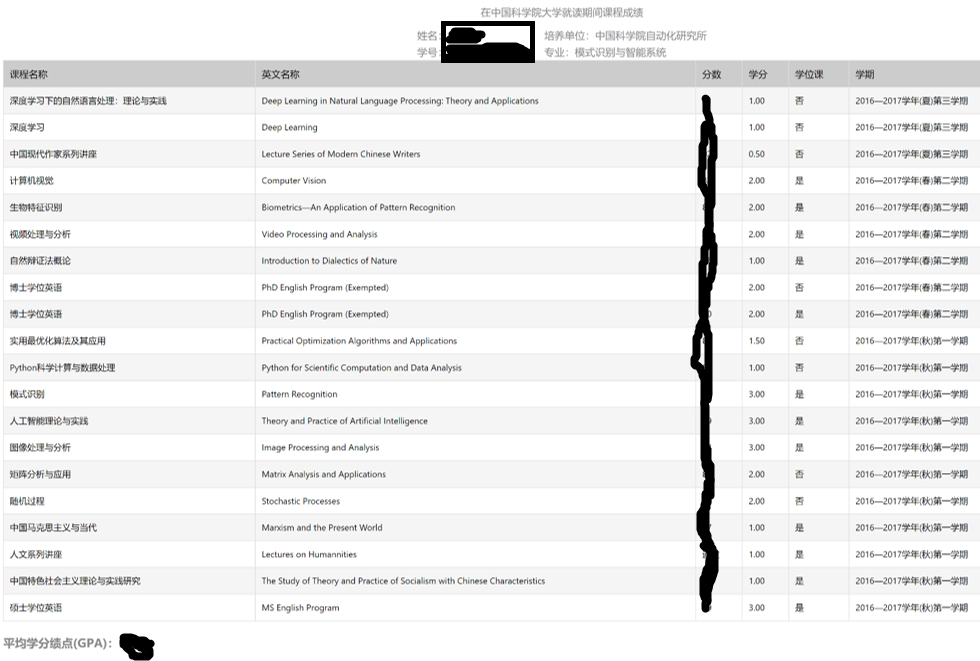
\includegraphics[width=0.99\linewidth]{Img/Others/score.png}
	\end{center}
	\caption{在中国科学院大学的已修课程和学分。
	}
	\label{fig:score}
\end{figure}
\begin{figure}[h]
	\begin{center}
		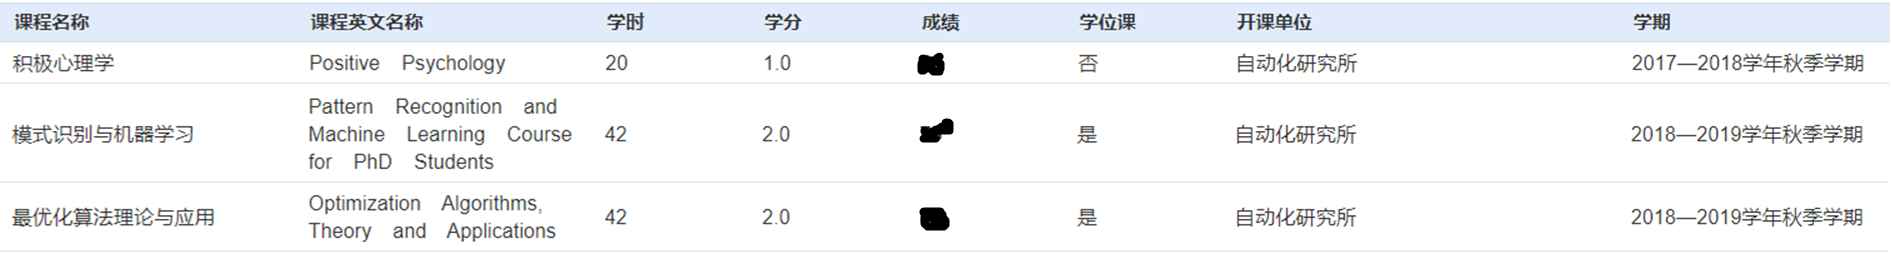
\includegraphics[width=0.99\linewidth]{Img/Others/score2.png}
	\end{center}
	\caption{在中国科学院自动化研究所的已修课程和学分。
	}
	\label{fig:score2}
\end{figure}

\chapter{学位论文开题存在的问题及回复}
学位论文开题时答辩老师主要关注的问题有两个。

一方面是xxx。回答如何解决。

另一方面是xxx。回答如何解决。

\chapter{学位论文撰写提纲}
\noindent 第一章\quad 绪论

介绍背景与意义,分析解决该任务存在的困难与挑战,并对本文的研究内容进行介绍。对学位论文的整体架构
进行描述。
\newline

\noindent 第二章\quad 国内外研究现状

介绍和本文相关的国内外研究现状。主要介绍xxx。
\newline

\noindent 第三章\quad 研究内容一

xxx。
\newline

\noindent 第四章\quad 研究内容二

xxx。
\newline

\noindent 第五章\quad 研究内容三

xxx。
\newline

\noindent 第六章\quad 总结与展望

xxx。
%---------------------------------------------------------------------------%
% main content

%-
%-> Appendix
%-
\cleardoublepage%
\appendix% initialize the environment
%-
%-> Backmatter: bibliography, glossary, index
%-% appendix content
%-
%-> Backmatter: bibliography, glossary, index
%-
\backmatter% initialize the environment
\intotoc*{\cleardoublepage}{\bibname}% add link to toc
\artxifstreq{\artxbib}{bibtex}{% enable bibtex
    \bibliography{Biblio/ref}% bibliography
}{%
    \printbibliography% bibliography
}
%%---------------------------------------------------------------------------%
%->> Backmatter
%---------------------------------------------------------------------------%
\chapter{作者简历及攻读学位期间发表的学术论文与研究成果}

\section*{已发表(或正式接受)的学术论文:}

{
\setlist[enumerate]{}% restore default behavior
\begin{enumerate}[nosep]
    \item xxx, 2014.
\end{enumerate}
}

\section*{申请或已获得的专利:}

(无专利时此项不必列出)

\section*{参加的研究项目及获奖情况:}

可以随意添加新的条目或是结构。

\chapter[致谢]{致\quad 谢}\chaptermark{致\quad 谢}% syntax: \chapter[目录]{标题}\chaptermark{页眉}
\thispagestyle{noheaderstyle}% 如果需要移除当前页的页眉
%\pagestyle{noheaderstyle}% 如果需要移除整章的页眉

感激casthesis作者吴凌云学长,gbt7714-bibtex-style
开发者zepinglee,和ctex众多开发者们。若没有他们的辛勤付出和非凡工作,\LaTeX{}菜鸟的我是无法完成此国科大学位论文\LaTeX{}模板ucasthesis的。在\LaTeX{}中的一点一滴的成长源于开源社区的众多优秀资料和教程,在此对所有\LaTeX{}社区的贡献者表示感谢!

ucasthesis国科大学位论文\LaTeX{}模板的最终成型离不开以霍明虹老师和丁云云老师为代表的国科大学位办公室老师们制定的官方指导文件和众多ucasthesis用户的热心测试和耐心反馈,在此对他们的认真付出表示感谢。特别对国科大的赵永明同学的众多有效反馈意见和建议表示感谢,对国科大本科部的陆晴老师和本科部学位办的丁云云老师的细致审核和建议表示感谢。谢谢大家的共同努力和支持,让ucasthesis为国科大学子使用\LaTeX{}撰写学位论文提供便利和高效这一目标成为可能。

\cleardoublepage[plain]% 让文档总是结束于偶数页,可根据需要设定页眉页脚样式,如 [noheaderstyle]
%---------------------------------------------------------------------------%
% other information
\end{document}
%---------------------------------------------------------------------------%

